\section{Probing the nucleus with tagged reactions} 

One of the popular methods to explain the EMC effect is that nucleons
are modified in the nuclear medium. This idea
triggered several experiments to measure the quasi-elastic 
process ($e+A \rightarrow e+p+X$). In this process, the 
elastic scattering occurs on a bound nucleon and allows to extract its modified 
form factor. One of the expectations from these measurements was to detect a change
in size of the bound nucleon compared to the free one. This has also motivated 
DVCS experiments, where a similar process is accessible, the so-called
incoherent nuclear DVCS ($e+A \rightarrow e+p+\gamma+X$). Results for these two 
channels are presented in Fig.~\ref{fig:QEincoh}, and show in both cases a 
significant deviation between the bound and the free nucleons. 
The difficulty with the interpretation of these measurements lies into the 
effect of final-state interactions. Indeed, the reaction products are likely
to re-interact with the remnants of the nucleus, and this affects significantly the
results. The calculation of these final state effect is complex and leads to large model 
uncertainties. 
Another problem is that in the calculation of these processes, it is important
that the initial and final-state nucleons are the same. This cannot be guaranteed
in a nucleus where one can have a off-shell nucleon in the initial state or 
have processes where a charge is exchanged and a neutron becomes a proton. For
these reasons, the debate remains open around 
the interpretation of the data on bound nucleon scatterings~\cite{Benhar:2006wy}.

\begin{figure}[tbp!]
\center
%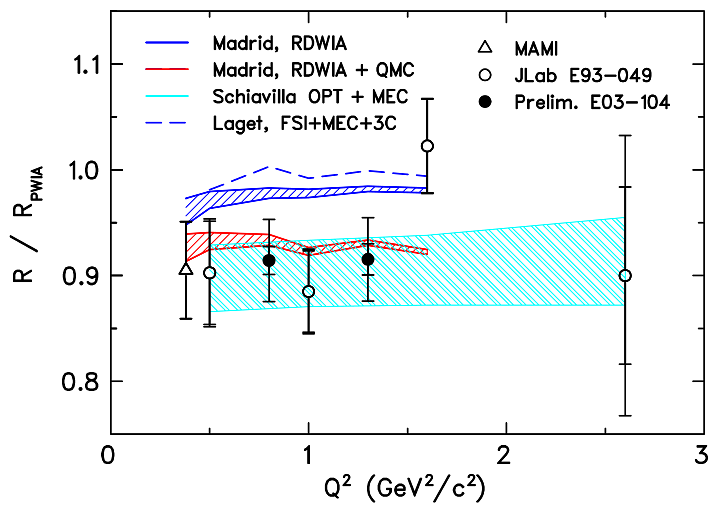
\includegraphics[width=7.6cm]{fig/ModifiedFF.png}
%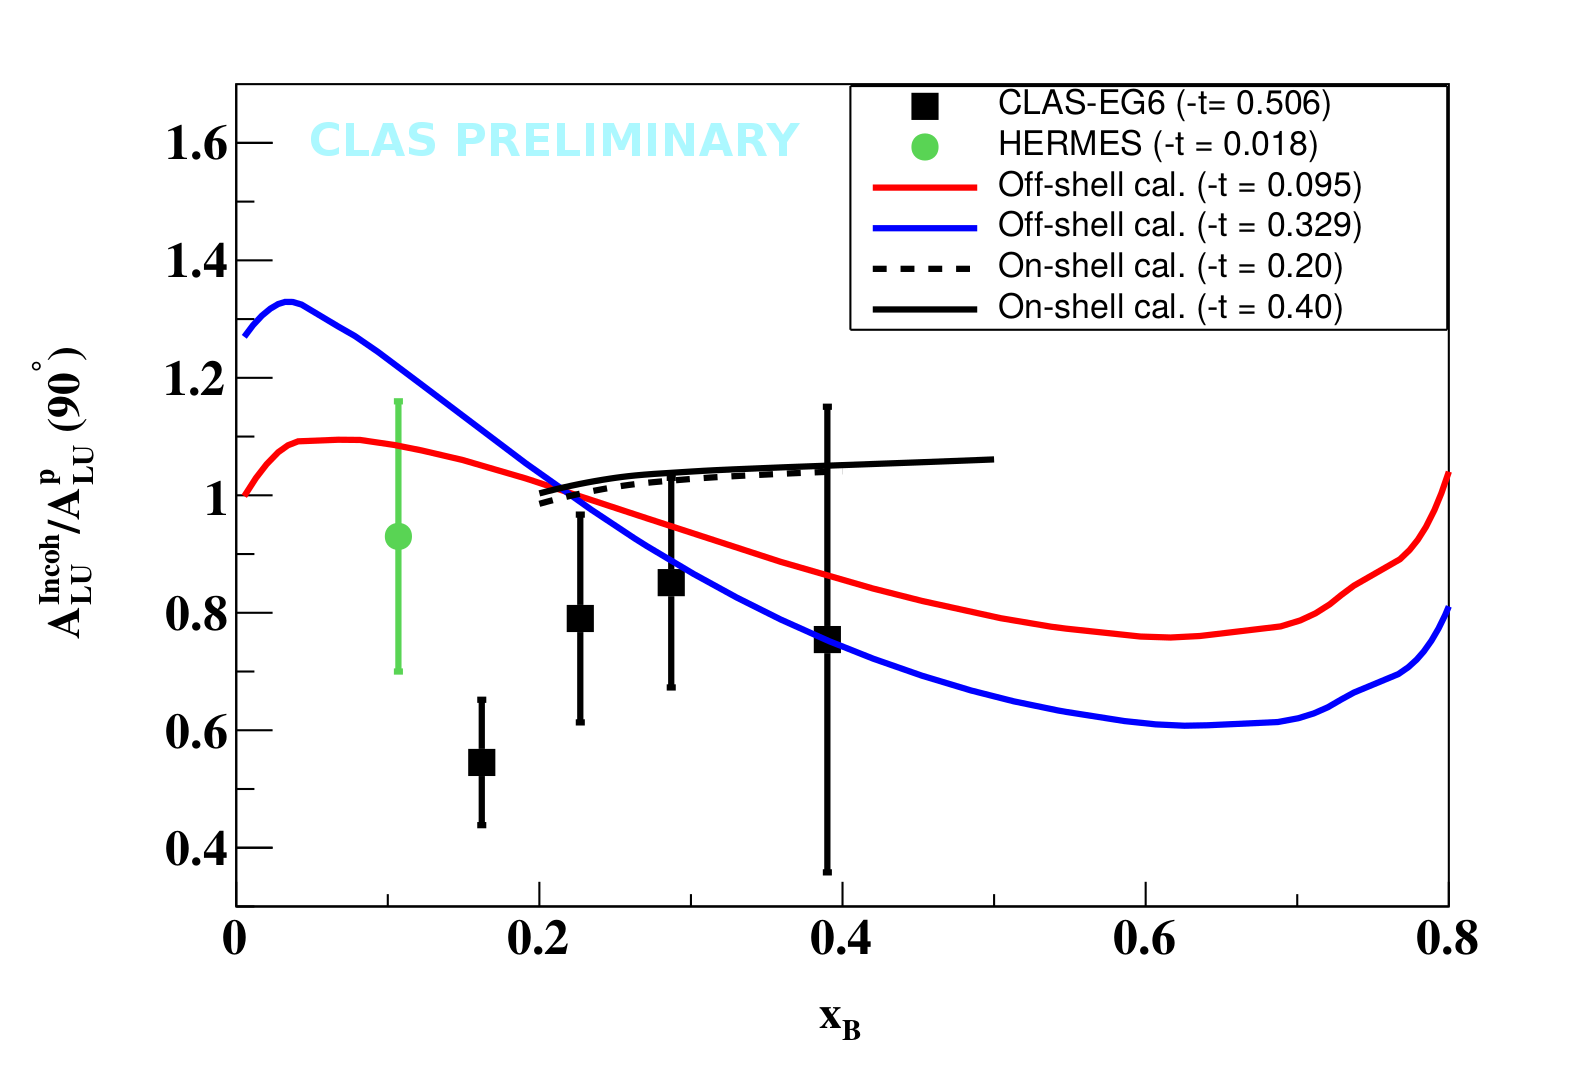
\includegraphics[width=8.5cm]{fig/ALU_ratioInc_x_shortscenrario.png}
\caption{Left: results of \cite{Strauch:2002wu} for the quasi-elastic form factor relative to
the plane wave impulse approximation. Right: CLAS preliminary results 
for the beam spin asymmetry in incoherent nuclear DVCS relative to the free proton DVCS.}
\label{fig:QEincoh}
\end{figure}

The solution to these problems is the tagging method, in which the nuclear fragments
are detected as described in Fig.~\ref{fig:tag} for the simplest case, deuterium.
In this process ($e+D \rightarrow e+p_s+X$), the high-energy electron is measured
together with the low-energy proton. The measurement of the proton in the backward 
direction ensures that it was not part of the hard interaction, thus noted with 
the $s$ subscript for spectator, and transforms the deuterium into 
an effective neutron target. First results of such a measurement
have been reported in~\cite{Baillie:2011za} with the goal to extract the structure
function of the neutron. We show in Fig.~\ref{fig:wstar} a result of this experiment
comparing the invariant mass obtained with and without the tagging method. It is 
clear that the tagging method gives a much better resolution of the structure 
present in the invariant mass distribution. Similarly to the measurement presented in 
the previous section, the main result of this experiment was however limited by the lack
of statistics. Yet, this successful measurement of a tagged process opens the way for more
experiments of the same kind in the future. 

\begin{figure}[htbp!]
\centering
\begin{minipage}{.48\textwidth}
  \centering
%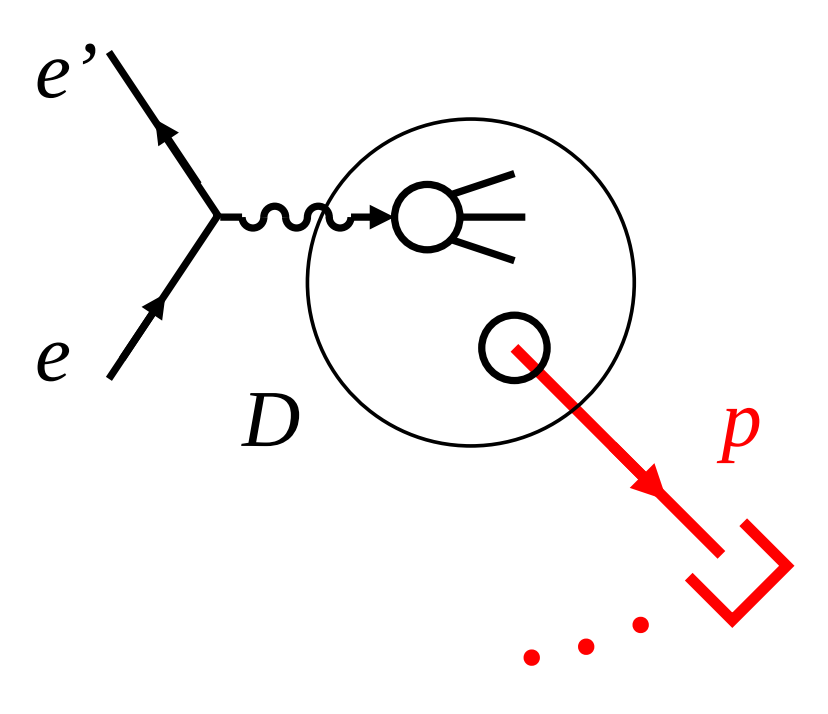
\includegraphics[width=6.1cm]{fig/Tagging.png}
\caption{Schematic of a tagged measurement on deuterium to obtain an effective
neutron target. Here the scattered electron $e^\prime$ and the proton $p$ are detected.}
\label{fig:tag}
\end{minipage}%
\hfill
\begin{minipage}{.48\textwidth}
  \centering
%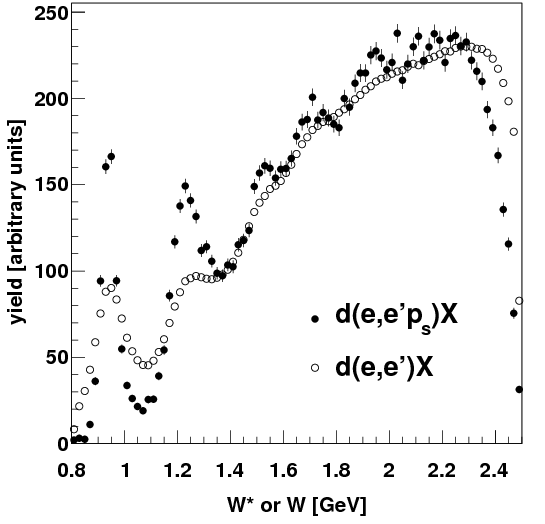
\includegraphics[width=6.1cm]{fig/Wstar.png}
\caption{Neutron-electron invariant mass obtained from tagging (full points) compared 
to the invariant mass obtained
from deuterium data (hollow points)~\cite{Baillie:2011za}.}
\label{fig:wstar}
\end{minipage}
\end{figure}

The nuclear tagging is the extension of the deuterium tagging to heavier nuclei, which
consists in measuring the reaction ($e+A \rightarrow e+(A-1)_s+X$), with
$(A-1)_s$ the spectator remnant of the nuclear target. This measurement is very 
interesting as it gives a direct information on which nucleon was hit by the 
deeply inelastic electron scattering in the nucleus. Also, by selecting 
low momentum backward emission of the $(A-1)_s$, we can suppress the 
final state interactions that are often a problem in such nuclear reactions. 
Detailed studies~\cite{CiofidegliAtti:2003pb,Alvioli:2006jd} have indeed shown 
that the final state interactions effects are minimized when the nuclear recoil
is detected in a backward angle relative to 
the virtual photon direction and maximized in perpendicular kinematics.
The detection of such recoil nuclei is however extremely challenging.

Tagging recoils has another interest in the quest to understand nuclear structure.
The kinematics of the nuclear remnants contain information on the
initial state of the nucleons in the nucleus. By performing at the same time the 
tagging and a deeply inelastic scattering, we probe simultaneously the nucleon and the 
quark structure of the nucleus. Tagging is therefore a unique tool to relate the EMC
effect to more classical nuclear effects and see if there is any correlation between
them. The more natural variable to use for these studies is the nucleon virtuality.
It can be calculated~\cite{CiofidegliAtti:2007ork} in the impulse 
approximation, where the nucleon momentum is exactly $\mathbf{p} = -\mathbf{P}_{A-1}$, 
giving:
\begin{equation}
v(|\mathbf{p}|, E) = \left (M_A - \sqrt{(M_A - m_N + E)^2 + \mathbf{p}^2} \right )^2 
                   - \mathbf{p}^2 - m_N^2,
\end{equation} 
where $E$ is the removal energy, $M_A$ the mass of the target nucleus
and $m_N$ the mass of the nucleon. The nucleon virtuality is a key 
observable to understand the nuclear quark and gluon structure,
as there are radically different predictions for its impact on the partonic structure.
Indeed, the descriptions of the EMC effect based on nucleon dynamic 
predict a strong correlation between virtuality and nucleon modification,
while the ones involving other hadronic degrees of 
freedom or mean field effects do not. 

Nuclear tagging measurements have never been performed in the past
on nuclei with $A>2$ due to detector limitations. Indeed, the radial TPC used 
for the experiments described above~\cite{Baillie:2011za}
is unable to differentiate isotopes and thus ensure the identification of 
nuclear remnants. There are plans at Jefferson Lab to remediate this issue
with the construction of a new detector to perform nuclear tagging measurements 
for the first time~\cite{Armstrong:2017zqr,Armstrong:2017zcm}.

